%\documentclass{templatearticle}
% -----------------------------------------------------------------------------
% User settings
% -----------------------------------------------------------------------------
%\myDoctype {}
%\myDivision {}
%\myTitle {}
%\mySubTitle {}
%\myAuthor {Rolf Koch}
%\myVersion {1.0}
%\myLanguage{german} % german or english
% -----------------------------------------------------------------------------
% Document: provide the two files abstract.tex and history.tex
% -----------------------------------------------------------------------------
%\begin{document}
%\setupLanguage            % setup configured language
%\setupWatermarks          % setup watermarks
%\printTitlePage{abstract} % include "abstract.tex"
%\printLeader{history}     % include "history.tex"
% -----------------------------------------------------------------------------
% Input user files with LaTex text sections
% -----------------------------------------------------------------------------

\documentclass[a4paper,oneside,notitlepage]{scrartcl}
\pdfcompresslevel=9



% define input encoding
\usepackage{ucs}
\usepackage[utf8x]{inputenc}



%German Language
\usepackage[ngerman]{babel}

\newcommand{\authors}{Rolf Koch, Sandro Ropelato, Michael Schwarz, \\Andreas Ruckstuhl, Christof Würmli}
\newcommand{\batitle}{Ligretto}


% for hyperlinks (TODO: configure hyperref package)
\usepackage{hyperref}
\hypersetup{
	colorlinks=true, 
	linkcolor=blue,
	citecolor=blue,
	filecolor=blue,
	menucolor=black,
	%   pagecolor=black,
	urlcolor=blue,
	breaklinks=true,
	pdfnewwindow=true,
	pdfauthor=\authors,
	pdftitle=VSY: \batitle
	%   pdfcreationdate=D:\pdfdate,
	%   pdfmoddate=D:\pdfdate,
	%   pdfsubject=pdfsuject,
	%   pdfkeywords=pdfkeywords
}

% to include a PDF directly into the generated document
\usepackage{pdfpages}

% Für Syntax Highlightings
\usepackage{listings}

\lstset{ %
language=Octave,                % the language of the code
basicstyle=\footnotesize,       % the size of the fonts that are used for the code
numbers=left,                   % where to put the line-numbers
numberstyle=\footnotesize,      % the size of the fonts that are used for the line-numbers
stepnumber=1,                   % the step between two line-numbers. If it's 1, each line 
                                % will be numbered
numbersep=4pt,                  % how far the line-numbers are from the code
backgroundcolor=\color{white},  % choose the background color. You must add \usepackage{color}
showspaces=false,               % show spaces adding particular underscores
showstringspaces=false,         % underline spaces within strings
showtabs=false,                 % show tabs within strings adding particular underscores
frame=single,                   % adds a frame around the code
tabsize=2,                      % sets default tabsize to 2 spaces
captionpos=b,                   % sets the caption-position to bottom
breaklines=true,                % sets automatic line breaking
breakatwhitespace=false,        % sets if automatic breaks should only happen at whitespace
title=\lstname,                 % show the filename of files included with \lstinputlisting;
                                % also try caption instead of title
escapeinside={\%*}{*)},         % if you want to add a comment within your code
morekeywords={*,...}            % if you want to add more keywords to the set
}

% for \colorbox
\usepackage{color}
% for graphics
\usepackage{graphicx}


% Big Tables across Pages
\usepackage{longtable}

\begin{document}
% titelseite
\begin{titlepage}
% \begin{center}
%  
\includegraphics[width=0.3\textwidth]{graphics/zhaw_title_logo.png} \\[1cm]
%
%  Bachelorarbeit \\ {\large \batitle} \\[1cm]
%
%  \includegraphics[width=0.4\textwidth]{graphics/infrasupport_logo.jpg}
%  \includegraphics[width=0.1\textwidth]{graphics/suw_logo.jpg}
% \end{center}

% standard titelseite:
\title{VSY Konzept \\ \batitle}
\author{\authors}
\date{24. April 2011}
\maketitle
\end{titlepage}

\pagenumbering{roman} 
%\input{0_zusammenfassung} \newpage
% Inhaltsverzeichnis
\renewcommand*\contentsname{Inhaltsverzeichnis}
\tableofcontents \newpage

\pagenumbering{arabic}
% content:
\section{Aufgabenstellung} 

Der Verlauf eines Ligretto-Spiel soll simuliert werden können. Um echten Zufall ins Spiel zu bringen, soll das Spiel über mehrere Maschinen verteilt werden

 \begin{itemize}
 \item Auf dem \textbf{Eingangsserver} lassen Sie einen Webserver laufen. Ein POST-Request auf den Server initiiert eine Ligretto-Simulation und liefert einen Link über den das Resultat per Polling abgholt werden kann. Das Resultat der Simulation wird  unter diesem Link als XHMTL-Seite präsentiert. Während der Berechnung wird eine Seite mit dem Text "in Bearbeitung" angezeigt.
 \item Eingangsparameter: Ausgangslage des Spiels (Verteilung der Karten) und implizit die Anzahl Spieler. Rückgabewert: Punkteverteilung für die Spieler
 \item Dieser Eingangsserver sei bereits komplett definiert. Sie erhalten die Daten aus dem POST-Request in der von Ihnen gewünschten Datenstruktur zur Weiterverarbeitung.
 \item Um das \textbf{Mischeln und Verteilen} der Karten müssen Sie sich nicht kümmern. Der Eingangsserver liefert ja bereits die Spielsituation genau vor Beginn des Spiels. Zu diesem Zeitpunkt sind die Karten verteilt und Spezialregeln (neue Karten bei >= 30 Punkte) sind bereits erfüllt. Aber Sie müssen dafür Sorgen, dass die \textbf{Clients die nötigen Informationen vom Eingangsserver} erhalten. Dies ist Abhängig von der von Ihnen gewählen Implementation.
 \item Ihnen stehen für die Simulation eine bestimmte \textbf{Anzahl Rechner} zur Verfügung. Die Rechner haben sich vorgängig beim Eingangsserver gemeldet, so dass er eine Liste der verwendbaren Clients hat und damit die Anzahl der verwendbaren Rechner kennt. Sie brauchen sich nicht darum zukümmern wie sich die Clients beim Server anmelden.
 \item Die \textbf{CPU-Leistung} ist nicht zu optimieren.
 \item Die \textbf{Berechnungszeit} ist  nicht zu optimieren.
 \item Beschreiben Sie den \textbf{Algorithmus} vollständig (Ax im Bewertungsmassstab). Sie beginnen ab dem Moment wo Sie die Daten vom Eingangsserver erhalten (in der von Ihnen definierten Datenstruktur). Das erste wird wohl die Verteilung der Daten auf die Client-Rechner seind.
 \item Beschreiben Sie alle verwendeten \textbf{Datenstrukturen} inklusive der Deklaration in Java oder C/C++.
 \item Beschreiben Sie die \textbf{Schnittstellen} als RPC x-File oder RMI-Interface. Nur die Schnittstellen die während dem Spiel benutzt werden sind hier verlangt.
 \item Die Anzahl Ziffern (1-10) und Frontfarben (4 verschiedene) sind unveränderliche Konstanten
 \item Wie \textbf{skalliert} das System mit Zunahme der Anzahl Spieler?
 \item Die restlichen Bewertungskriterien (wie Rechnerausfall etc.) können Sie weglassen
 \item Die \textbf{Spielstrategie} können Sie an eine Funktion KI auslagern. Wenn Sie also aus spieltechnischen Ueberlegungen eine Karte nicht legen wollen, obwohl es möglich wäre, so kann diese Entscheidung durch diese KI-Funktione ermittelt werden. Sie müssen allerdings die für die Entscheidung nötigen Informationen dieser Funktion zur Verfügung stellen. D.h. Sie müssen sich überlegen welche Informationen nötig sind und woher diese Informationen besorgt werden. Aber um die Implementation der Spieletheorie müssen Sie sich nicht kümmern.
\end{itemize}
	
	
% Beispiel um eine Grafik einzubinden
	
%\begin{figure}[hbt]
%  \centering
%  \includegraphics[width=0.65\textwidth,angle=0]{graphics/zhaw.png}
%  \caption{ZHAW Logo}
%  \hfill{} }
% \end{figure} \newpage
\section{Spielbeschreibung}

\begin{figure}[hbt]
  \centering
  
\includegraphics[width=0.45\textwidth,angle=0]{graphics/ligretto.jpg}
  \caption{Ligretto \hfill{} }
 \end{figure}

Ligretto ist ein Spiel bei dem es darum geht seinen eigenen Ligretto Stapel los zu werden bevor dies ein Gegner schafft. Der Ligretto Stapel besteht aus 10 verdeckten zufälligen Karten aus dem Kartenvorrat des Spielers. Der Kartenvorrat eines Spielers, auch Deck genannt, besteht aus 40 Karten. Die Karten sind von 1 bis 10 nummeriert und haben 4 Farben: Rot, Gelb, Blau und Grün. Es gibt keine doppelten Karten, das heisst jede Karte kommt nur genau einmal vor im Deck des Spielers.

\begin{figure}[hbt]
  \centering
  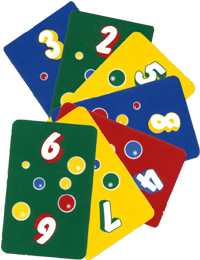
\includegraphics[width=0.20\textwidth,angle=0]{graphics/ligretto.png}
  \caption{Ligretto Karten \hfill{} }
 \end{figure}

Um ein neues Spiel vorzubereiten mischt jeder Spieler seinen Kartenstapel. Jeder Spieler zählt dann 10 Karten ab und legt diese verdeckt vor sich hin. Dies ist sein eigener Ligretto Stapel. Danach legt er 4 Karten von seinen restlichen Handkarten offen neben den Ligretto Stapel. Sobald alle Spieler soweit sind geht es los.

Der Spielablauf funktioniert nun wie folgt für jeden Spieler:
\begin{enumerate}
\item Der Spieler schaut die offen vor sich liegenden Karten an.
\item Der Spieler prüft die Stapel an Karten in der Mitte des Spielfelds. 
\item Der Spieler versucht nun eine Karte zu finden, die eins höher ist als die oberste Karte eines Stapels und die selbe Farbe besitzt. Ist dies der Fall, so darf er seine Karte nehmen und oben auf diesen Stapel legen.
\item Wenn diese gelegte Karte eine der 4 offen vor sich liegenden Karten gewesen ist, dann darf der Spieler die oberste Karte vom Ligretto Stapel aufdecken und anstelle der soeben gelegten Karte vor sich hin legen.
\item Wenn eine 1er Karte verfügbar ist, darf damit ein neuer Stapel in der Mite des Spielfelds eröffnet werden.
\item Wenn mit den offenen Karten keine Aktionen durchgeführt werden können darf der Spieler von seinen restlichen Handkarten 3 Karten verdeckt abzählen und diese umdrehen und vor sich auf den Ablagestapel legen. Existiert noch kein Ablagestapel so legt er die 3 Karten neben seine bereits vor sich liegenden Karten und eröffnet somit seinen Ablagestapel. Beim Ablagestapel darf nun jeweils die oberste Karte ebenfalls gespielt werden.
\item Sollte weiterhin keine Karte gelegt werden können, so wiederholt der Spieler Punkt 6 und legt immer 3 Karten oben auf den Ablagestapel, bis er keine Handkarten mehr in der Hand hält. Ist dies der Fall, so nimmt der Spieler den Ablagestapel wieder als Handkarten auf und fängt von vorne an.
\end{enumerate}

Sobald ein Spieler die letzte Karte seines Ligretto Stapels aufgedeckt hat, ruft er Ligretto Stop, das Spiel wird beendet und es wird abgerechnet.

Bei der Abrechnung bekommt jeder Spieler Punkte für sich selber. Die Abrechnung läuft wiefolgt ab:


\begin{enumerate}
\item Jeder Spieler zählt die noch vorhandenen Karten auf dem eigenen Ligretto Stapel. Für jede Karte auf dem Ligretto Stapel bekommt er zwei Minuspunkte.
\item Die Karten auf dem Spielfeld werden nun wieder nach Farbe auf der Rückseite sortiert. Jeder Spieler erhält seine Karten zurück und zählt diese. Für jede gelegte Karte bekommt der Spieler einen Pluspunkt.
\item Die Punkte werden nun notiert und  jeder Spieler bereitet sich für die nächste Runde vor.
\end{enumerate}  \newpage
\section{Problemanalyse}   %wo liegen die Probleme oder Schwierigkeiten in einer Ligrettosimulation mit verteilten Systemen?

%allgemein, was muss analysiert werden

Als Aufgabe gilt es, den Ablauf, der durch die Spielregeln festgelegt ist, anhand folgender Gesichtspunkte in einen Algorithmus umzusetzen:

\begin{enumerate}
	\item Der Spielablauf muss den Spielregeln entsprechen und die KI-Algorithme, welche die Mitspieler simulieren, sollten nur an Informationen über den Spielablauf gelangen, welche auch ein menschlicher Spieler gelangen würde.
	\item Der Spielablauf sollte möglichst fair sein. D.h. bis auf den Zufall, der durch das Mischen der Karten ins Spiel gelangt, sollten alle Mitspieler gleichgestellt sein.
	\item Die verwendeten Algorithmen und Schnittstellen sollten möglichst gut mit der Anzahl Mitspieler skalieren, unter Betrachtung der benötignen Rechenzeit und Netzerkkapazität.
\end{enumerate}

Folgende Punkte werden bei der Herleitung des Algorithmus nicht betrachtet:

\begin{enumerate}
	\item Alle Mitspieler müssen sich an die Spielregeln halten, insbesonder in Teilen des Ablaufs, die im Spiel mit menschlichen Spielern nicht überwacht werden können. Dazu gehör z.B. das regelkonforme Ablegen der Handkarten beim suchen einer passenden Karte.
	\item Die beiligten Server versenden nur Nachrichten an Server, mit denen sie laut dem Alogrithmus kommunizieren dürfen.
	\item Die eingesetzte Software und Hardware darf keine Fehler aufweisen und der Netzerkverkehr darf nicht gestört oder unterbrochen werden. D.h. z.B. keine Pakete dürfen verloren gehen.
\end{enumerate}

%Für die letzten beiden Punkte wird anschliessend eine Diskusion gegeben, inwiefern der Alogorithmus und die Schnittstellen angepasst werden müssten, um ...

\subsection{Systemgrenzen}

%welche teile des algorithmus laufen wo

Damit die Laufzeit eines Spiels nicht, oder nur schwach, mit der Anzahl Spieler wächst, muss die Anzahl verwendeter Server linear mit der Anzahl Mitspieler wachsen können. Deshalb ist es notwendig und sinnvoll für jeden Mitspieler mindestens einen, separaten Prozess zu Verwenden.

Da ein einzelner Spieler jedoch zu jeder Zeit immer nur eine Aktion ausführen darf (siehe Spielregeln), ist eine Aufteilung eines einzelenen Spielers in mehrere Prozesse nicht sinnvoll.

Zur Überwachung des gesammten Spiels, sowie dessen Aufbau und Abbau, wird ein separater Prozess verwendet. Da der Überwachende Prozess nur vor Spielbeginn und nach Beendigung des Spiels eine Aufgabe hat, dessen Komplexität mit der Anzahl mitspieler wächst, ist eine Aufteilung deiser Aufgaben in mehrere Prozesse zwar erwägenswert, aber nicht von oberster Priorität.

% TODO: Nomenklatur für den Überwachende Prozess und Mitspieler-Prozesse

Zusammengefasst:

\begin{enumerate}
	\item Ein Prozess zur Überwachung des Spiels (Aufbau und Abbau).
	\item Ein Prozess pro Mitspieler, welche alle Aktionen des jeweiligen Mitspielers durchführt.
\end{enumerate}

\subsection{Verteilung}

%welcher state ist wo

Bei der Betrachtung der Verteilung des Zustandes gibt es drei Arten von Objekten:

\begin{enumerate}
	\item {\bf Zustands-Objekte} verkörpern den veränderlichen Zustand eines Spiels. Die Eigenschaften dieser Objekte sind somit mutierbar. Für diese Objekte ist immer genau ein Prozess zuständig und diese Objekte werden auf andere Prozesse verschoben oder kopiert.
	\item {\bf Token-Objekte} werden zur Kommunikation verwendet und sind nicht weränderbar. Token-Objekte können zwischen den Prozessen verschoben werden, jedoch ist immer nur genau ein Prozess für ein jeweiliges Token-Objekt verantwortlich.
	\item {\bf Transiente Objekte} werden zu Kommunikations-Zwecken und zur unterstützung der Algorithmen erstellt und aufbewahrt. Wenn ein transientes Objekt an einen anderen Prozess versendet wird, dann besitzen beide Prozess eine eigene Kopie des Objektes.
\end{enumerate}

Die folgenden Token-Objekte können identifiziert werden:
\begin{enumerate}
	\item Spielkaren: Zu beginn des Spieles wird für jede Spielkarte, welche in einen realen Ligretto-Spiel verwerdet würde, ein Spielkarten-Objekt erstellt.
\end{enumerate}

Folgende Zustands-Obekte können identifiziert werden:
\begin{enumerate}
	\item Handkarten-Stapel
	\item Ausgelegte Karten vor dem Mitspieler
	\item Stapel auf dem Spieltisch
	\item Mitspieler
	\item Überwachender Prozess
\end{enumerate}

Zur Kommunikation werden folgende Transiente Objekte erstellt:
\begin{enumerate}
	\item Start- und Stop-Signale.
	\item Stapel mit gemischten Karten, welche vom Überwachenden Prozess and die Mitspieler verteilt werden.
	\item ...
\end{enumerate}

\subsection{Kommunikation}

%für was wird wie kommuniziert

z.B. wird {\tt LigrettoStopp()} aufrerufen.




%Um das Problem des Ligretto Systems zu verstehen definieren wir in erster Linie mal Assets, die es zu verwalten gilt. In einem zweiten Schrit 




\subsection{Concurrency-Problem}

%was gibt es für deadlocks, 

\subsection{Zuverlässigkeit}

%was passiert, wenn nachrichten verloren gehen (geht nicht, RMI ist synchron (hähä, wissen wir noch gar nicht ...))
%was passiert, wenn clients oder der server abstürzen
 \newpage
\section{Lösungsansatz} 

Client 1 hat vom Server Client 2 bis Client 7 als Nachbarn zugewiesen bekommen. Als erstes selektiert der Client 1 eine Karte und versucht diese bei sich selbst Legen. Gelingt dies nicht, versucht er die Karte bei einem seiner 6 Nachbarn zu legen, indem er ihnen die Karte übergibt und, falls sie gelegt werden konnte, eine Erfolgsmeldung (\textit{true}) oder ansonsten eine Misserfolgsmeldung (\textit{false}) zurückbekommt. Konnte er die selektierte Karte legen, wird diese gelöscht und eine neue Karte wird selektiert, mit welcher wieder von vorne begonnen wird. Das Beispiel von Client 1 ist representativ für alle Clients. 

\begin{figure}[hbt]
  \centering
  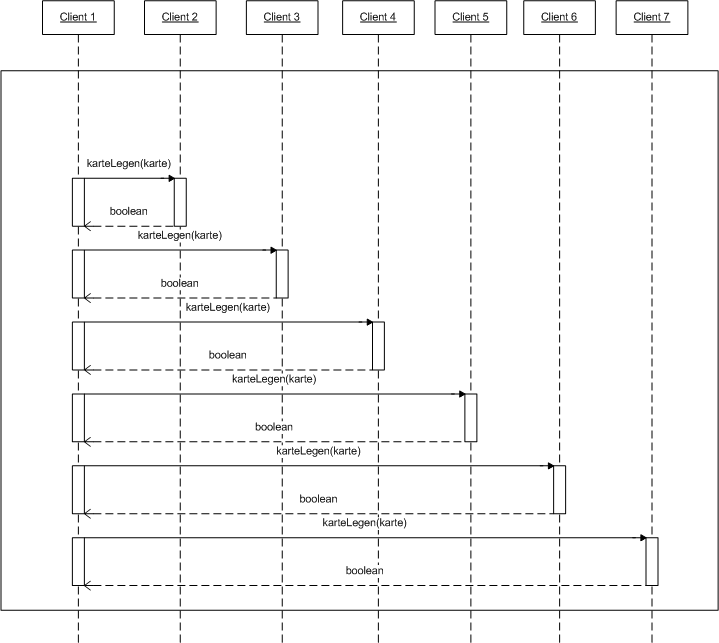
\includegraphics[width=0.90\textwidth,angle=0]{graphics/Kartenlegen_Sequenzdiagramm.png}
  \caption{Sequenzdiagramm: Kartenlegen}
\end{figure}

Dadurch, dass nicht zuerst der Status der Spiel-Stapel der Nachbarn abgefragt werden muss und danach versucht wirde eine Karte zu lege, ist die Kommunikation auf den Versuch einfach eine Karte zu legen minimiert. Es wird also nur eine Karte übertragen und entweder "true" für den Erfolg oder "false" für den Misserfolg zurückgegeben.
Zudem verwaltet jeder Spieler (Client) seine eigenen Spiel-Stapel vor sich. Diejenigen die er selbst erstellt hat mit einer Eins. Der Spieler muss also nur maximal 4 Spiel-Stapel verwalten auf die andere Spieler (Clients) Zugriff haben. 
Auch ist die anzahl Spieler die auf diese Spiel-Stapel Zugriff haben beschränkt, indem jeder Spieler nur 6 Nachbarn bekommt, mit denen er spielen kann. Wenn diese Nachbarn Sinnvoll verteilt sind, also das heisst solche Spieler die Lokalisationsmässig nahe beieinander liegen auch Nachbarn sind, findet die Kommunikation nur lokal statt und somit wirde ebenfalls die Kommunikation über das globale Netz minimiert.
% Bewertungsmasstab:
% - Ist der Algorithums zur Lösung der Teilafugaben nachvollziehbar? (3 Punkte)

%    - Der Teil für die Initialisierung/Setup wird nicht hier bewertet
%    - 2 Punkte für die komplexeren Komponenten (z.B. die "Clients")
%    - 1 Punkt für die weniger komplexen Komponenten
%    - Das umfasst auch die Kommunikation (wann kommuniziert wer mit wem)

% Nutzung der Ressourcen / Performance
%  -  Ist die Kommunikation minimiert?
%  -  Ist der Bedarf an Memory / Storage sinnvoll? \newpage
\section{Spiel Algorithmus} 

\subsection{Strategie}

\subsection{KI}

Ist nicht direkt teil unseres Konzepts, aber wir müssen der KI gewisse Informationen zur verfügung stellen damit sie überhaupt operieren kann.

Dazu gehören:

Spiel Start Signal
Stapel in der mitte des Spielfelds
Die Handkarten des Spielers
Das Legen einer Karte auf einen Stapel (Erfolgreich oder nicht)
Spiel End Signal
Punkte Abrechnungs Informationen

\subsection{Ablaufdiagramm}

1. dä Server verwaltet diä KartenStapel wo i dä mitti vom spielfeld sind
			2. dä Server hät am afang pro spieler 40 karten wo vorsortiert sind diä muäs är irgendwiä äm jewiligä spieler übergä
			3. sobald diä karte übergä sind übernimmt dä client d kontrolle über diä chartene
			4. dä client baut sin ligretto stapel, + sini 4 offne charte und seit dänn am Server, dass er Ready isch
			5. dä server wartet bis alli Ready sind und macht dänn äs Startsignal
			6. jede client fangt jetzt a regelmässig dä zuästand vo dä Stapel i dä Mitti abzfragä und versuächt sini chartene z spiele.
			7. Wenn er ä möglichkeit gseet versuächt er ä charte am Server z übergä für än gwüssä Stapel. Er wartet bis dä Server meldet ob das klappt hät oder nöd
			8. Sobald das klappt hät macht er wiiter, wänns nöd klappt hät chunt er vom Server sini Charte zrugg über und muäs si wieder detä härä legä wo si gsi isch.
			nachdem ein spieler sin ligretto stapel fertig hät macht er irgend äs Ligretto Stop signal. dä Server leitet das wiiter a alli spieler und returnt no alli charte wo erst nach däm ligretto stop signal acho sind.
			jede spieler zellt jetzt sin ligretto stapel und meldet diä zahl an Server
			dä Server sortiert alli karte, zellt si und verrechnet jetzt diä pünkt.
			
\begin{figure}[hbt]
  \centering
  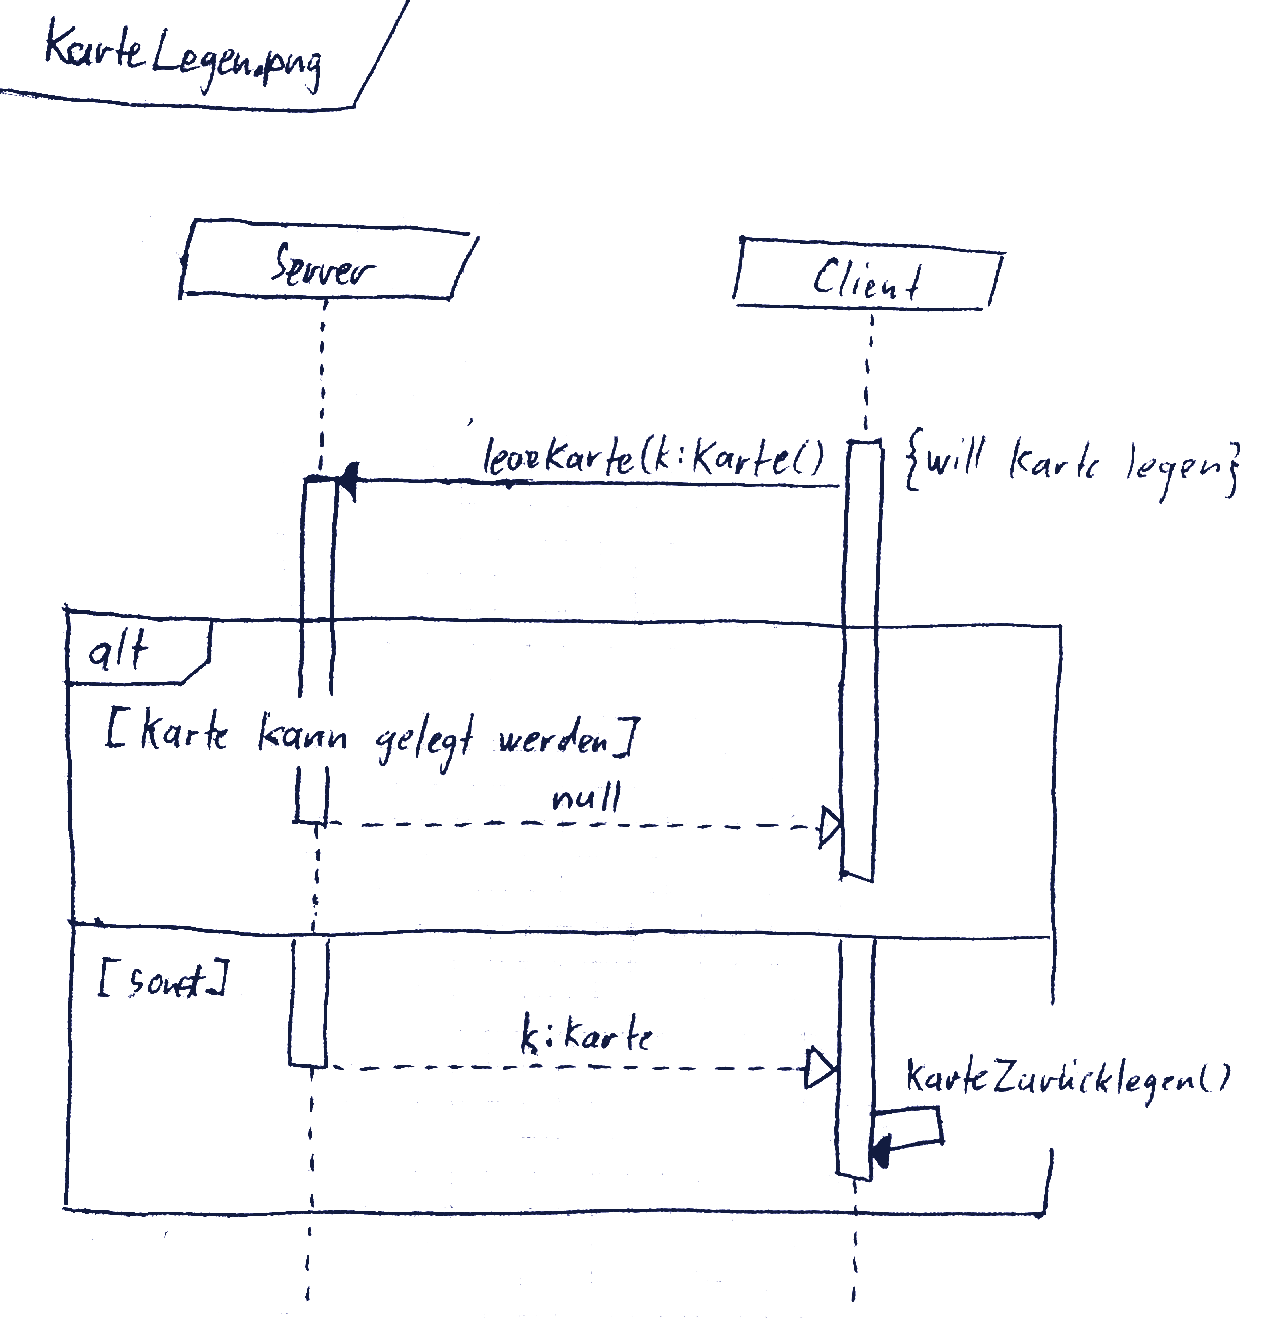
\includegraphics[width=0.80\textwidth,angle=0]{graphics/KarteLegen.png}
  \caption{Sequenzdiagramm zum Legen einer Karte [Papier und Stift FTW] \hfill{} }
 \end{figure}
 
 \subsection{Graphik}
 \begin{figure}[hbt]
  \centering
  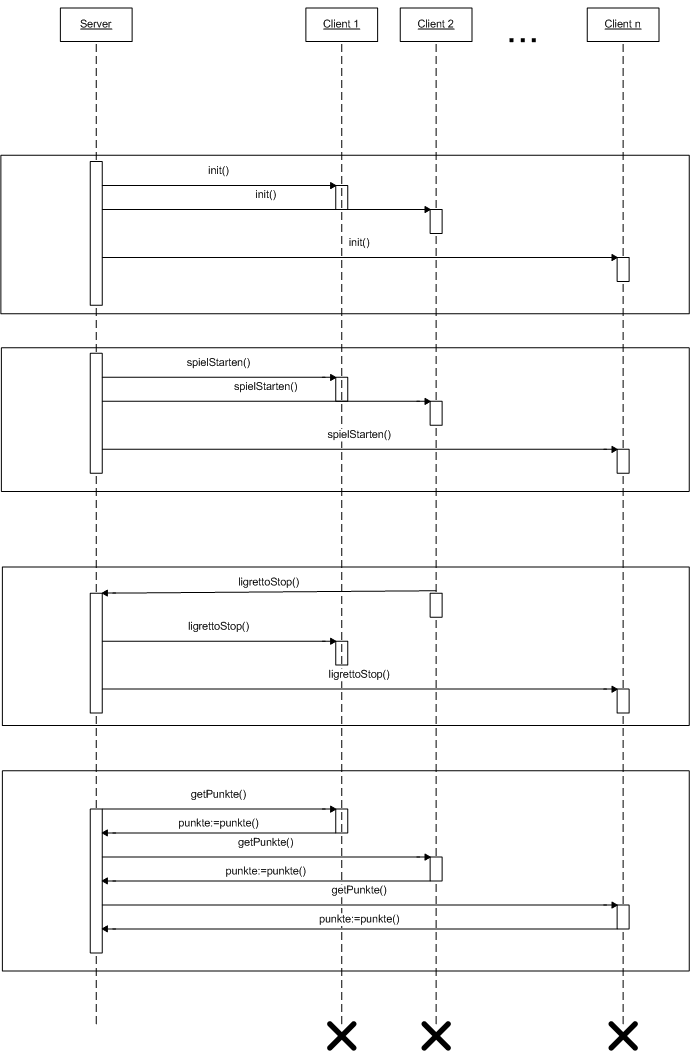
\includegraphics[width=0.60\textwidth,angle=0]{graphics/Spielablauf_Sequenzdiagramm.png}
  \caption{Sequenzdiagramm für den Spielablauf [Visio FTW] \hfill{} }
 \end{figure}

 \newpage
\section{Datenstrukturen} 

\subsection{Klassendiagramm}

Karten

Handkarten

Kartenstapel

Collection aller Kartenstapel

Start Signal

End Signal

Abrechnungs Daten \newpage
\section{Schnittstellen} 

\subsection{RMI-Interfaces}

\subsubsection{Client}


\lstinputlisting[language=Java]{RemoteClient.java}


\subsubsection{Server}

\lstinputlisting[language=Java]{RemoteServer.java}


% Für die Direkte eingabe des Codes kann man das hier benutzen:
% \begin{lstlisting}[language=Java]
% \end{lstlisting}


 \newpage
\section{Erwartetes Ergebnis}  \newpage


% Appendices

%\appendix

%\section{Quellenverzeichnis}
% TODO: BiBTex??
%\bibliographystyle{unsrt}
%\bibliography{quellenverzeichnis}

\end{document}